\begin{description}

\item[Debuggee]
	The piece of software for which we want to analyze cache usage. The term debuggee is used because it’s run with valgrind which is usually used for debugging.
\item[Matrix]
	A matrix is, in our case, an area of the memory which the debuggee has marked to contain data that is to be analyzed by our software. 
\item [Access]
	An access is an event generated for the debuggee. It marks loading or storing data to the main memory with a specific address.
\item[Relative Access]
	We are matching memory accesses to matrices and compute coordinates from that. For each access and it's previous access, a difference is coputed, and that is called a relative access. \newline
	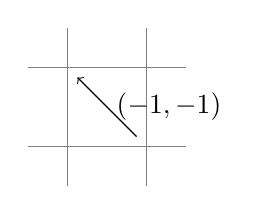
\begin{tikzpicture} %Tikzpictures are going to be fun. Our coordinate systems diverge...
		\draw [color=gray] (-0.5,-0.5) grid (1.5,1.5);
		\node (frst) at (1,0) {}; %nth access
		\node (scnd) at (0,1) {}; %n+1-th access
		\draw [->] (frst) -- (scnd) node [midway,right,draw=none] {$(-1,-1)$};
	\end{tikzpicture}
\item[Pattern]
	A pattern is an ordered set of relative accesses. These accesses have been observed subsequently multiple (to be exact: at least two) times. It is not guaranteed that the first access of a pattern always occures first. Patterns can't tell you anything about when or in which compositions they occur
\item[Sequence]
	When scanning for patterns in the access stream, a series of consecutive accesses is often accounted to one pattern. The length of this series and what happens next is bundled into a sequence.
\end{description}
